\documentclass{article}

\usepackage{amsmath,amsthm,amsfonts,amssymb,bm}
\addtolength{\textheight}{5.0cm}
\addtolength{\voffset}{-3.5cm}
\addtolength{\hoffset}{-2.5cm}
\addtolength{\textwidth}{4.0cm}

%\allowdisplaybreaks

\usepackage{amsmath}
\usepackage{subeqnarray}
%\usepackage{mathrsfs}
\usepackage{color}
\usepackage{url}
%\usepackage{ulem}
\usepackage{indentfirst}
%\usepackage{textcomp}
%\usepackage{graphics}
\usepackage{graphicx}
%\usepackage[hang,small,bf]{caption}
%\setlength{\captionmargin}{50pt}
\graphicspath{{Figures/}}

%\usepackage{tikz}
%\usetikzlibrary{mindmap,trees}

\begin{document}
\title{Power Spctrum \& Its Evolution}
\author{MA Lei}
\maketitle



\hrule\vspace{1pt}\hrule
\begin{center}
\mbox{{\bf Progress Note}} \\
\vspace{0.5em}
\mbox{2011-11-30}
\end{center}
\hrule


\section{Power Spectra \& Gauge}
\newtheorem{defination}{Defination}[section]
\newtheorem{convention}{Convention}[section]

\subsection{Defination}

\begin{convention}[Line Element]
$$\mathrm ds^2=-a^2(1+2AY)\mathrm d\tau^2-a^2BY_j\mathrm dt\mathrm dx^j+a^2(\gamma_{ij}+2H_LY\gamma_{ij}+2H_TY_{ij})\mathrm dx^i\mathrm dx^j$$
\end{convention}

\iffalse
\begin{figure}[!htpb]
\centering
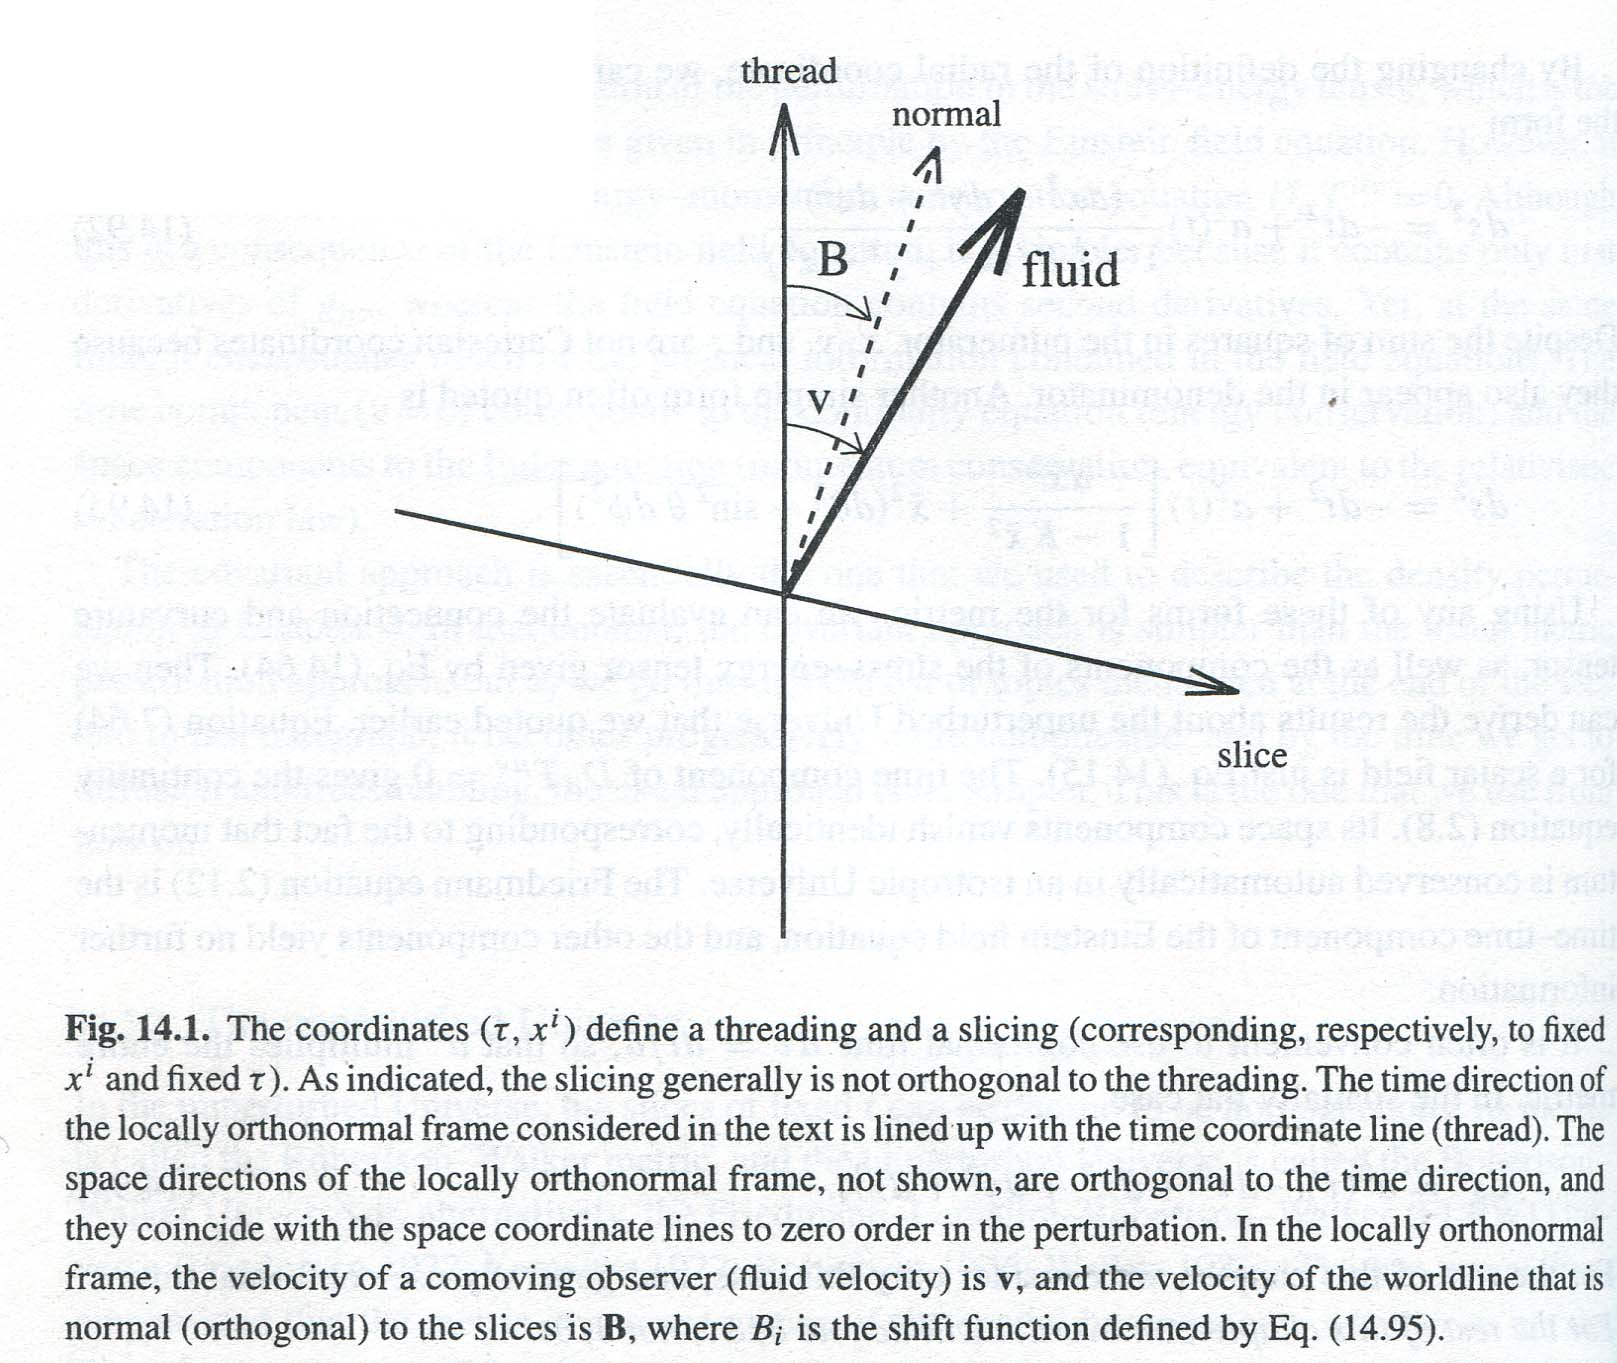
\includegraphics[width=460pt]{GaugeIntrepertation1.jpg}
\caption{Interpretating Gauge. B is for }\label{fig:Gauge1}
\end{figure}
\fi




\begin{defination}[Power Spectrum]
Power spectrum in k space is defined as \\
$$P(k)=\left<\left|D_g(\vec k)\right|^2\right>$$
\end{defination}
in which $\Delta_g=\delta_k+3(1+w)\mathcal R$ stands for the energy density contrast in flat slicing, i.e., $\mathcal R\equiv H_L+\frac 1 3 H_T=0$.{\footnote{I have no idea why Ruth Durrer define it this way. $D_g$ is some kind of energy density contrast when the curvature $\mathcal R$ vanishes. Maybe this curvature independent defination is better than other curvature dependent energy contrast definations.}}

Some dimensional analysis will be done in the following.

Energy density contrast in real space is defined to be dimension free, that is to say, energy density contrast in fourier space have the demension of $[L]^3$ since $[\delta(\vec r)]\sim [\delta_k][\mathrm d^3k]$ within which quantities in square brackets stand for their dimension.

Problem is, quantities that are not dimension free will lead to "discrepancies and floating-point errors in computations"{\footnote{http:\slash\slash www.ocf.berkeley.edu/~adriand/class/files/p228/11.pdf  (Page 3).}}. Then most people are glad to use the dimensionless power spectrum{\footnote{The role of $(2\pi)^3$ in Fourier transformation can be reversed. Then other possible defination of such a dimensionless power spectrum is to time a $(2\pi)^3$ factor on the following one.}},
\begin{equation}
\Delta^2_k\equiv \frac{4\pi k^3 P(k)}{(2\pi)^3}
\end{equation}

When we are talking about matter power spectrum we always use a dimensionless one from now on. {\color{red}(CMBEASY plotted $P^{(s)}_k=\frac{k^3\left<\left|\delta\right|^2\right>}{2\pi^2}$ as the sychronous gauge power sepctrum while $P^{(i)}_k=\frac{k^3\left<\left|\Delta_g\right|^2\right>}{2\pi^2}$. Michael Doran called this the gauge ambiguities. In other words, Michael Doran use different definations for different gauge! He mentioned that "Had I plotted the synchronous gauge dnsity contrast infered from the gauge invariant one, the two curves would of course fall on top of each other.{\footnote{http\slash\slash cosmocoffee.info/viewtopic.php?t=204\&highlight=astroph+0503277}}" The invariant power spectrum $P^{(i)}_k$ reduces to sychronous gauge power spectrum $P^{(s)}_k$) when we consider power sepctrum for cdm under horizon after LSS. From this point of view, this defination is not so treachery and it is not bad to stick to Micheal Doran's defination.)} 

A calculation in {\it Cosmology (2008)} by Weinberg shows that under adiabatic initial condition and with spectral index $n_s=1$,
$$P_k\equiv \Delta^2_k={\text{Const.}}\cdot k T^2(k).$$

Trnasfer function $T(k)\sim \frac{1}{k^2}$ ($\rightarrow P_k\sim \frac{1}{k^3}$) when $k$ is very large and $T(k)\sim {\text{Const.}}$ ($\rightarrow P_k\sim k$) when $k$ is very small.{\footnote{Weinberg uses different notations. He uses $q$ for comoving wave number while here we are using $k$ for that. \\ His calculation of this power spectrum is under sychronous gauge.}}

To get a intuitive view of Weinberg's calcuation, we consider the following statements. 

Given a HZ initial power spectrum $P_k=Ak$, the current power spectrum has the same value at small wave number (shown in Figure \ref{fig:powerspectrum1}{\footnote{\url{http://www.itp.uzh.ch/courses/phy513}}}).
\begin{figure}[!htpb]
\centering
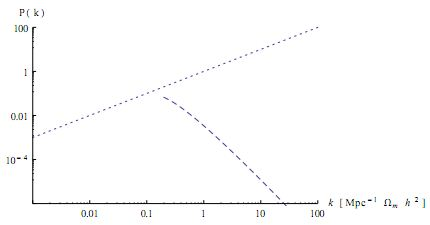
\includegraphics[width=300pt]{PowerSpectrum_CDM.jpg}
\caption{Current power spectrum keeps the initial value at small wave number.}\label{fig:powerspectrum1}
\end{figure}

 


As a reminder, $P(k)$ with $[Length]^3$ dimension can also be calculated easily by dividing $P_k$ by $k^3$.


\iffalse
\subsection{Gauge \& Evolution}

\paragraph{Invariant Gauge}

Evolution equation for matter outside of the horizon is
\[\ddot\Delta+2\frac{\dot a}{a}\dot\Delta-\frac 3 2 \left(\frac {\dot a}{a}\right)^2\Delta=0\]

This equation is exactly the same as the subhorizon evolution equation of matter perturbation in sychronous gauge. Then the power spectrum outside of the horizon in invariant gauge should have the same trend as the evolution of power sepctrum in sychronous gauge, i.e., 

\fi





\iffalse

\section{Appendix}


\subsection{Power Spectrum \& Correlation Function}
Power Spectrum{\footnote{Large-scale structure of the Universe and cosmological perturbation theory, F. Bernardeau, S. Colombi, E. Gaztanaga, R. Scoccimarro, Physics Report 367 (2002) 1-248. (Page 32).}}


\fi


\end{document}